%%%%%%%%%%%%%%%%%%%%%%%%%%%%%%%%%%%%%%%%%
% Stylish Curriculum Vitae
% LaTeX Template
% Version 1.1 (September 10, 2021)
%
% This template originates from:
% https://www.LaTeXTemplates.com
%
% Authors:
% Stefano (https://www.kindoblue.nl)
% Vel (vel@LaTeXTemplates.com)
%
% License:
% CC BY-NC-SA 4.0 (https://creativecommons.org/licenses/by-nc-sa/4.0/)
%
%%%%%%%%%%%%%%%%%%%%%%%%%%%%%%%%%%%%%%%%%
% !TEX program = xelatex
\documentclass[a4paper, oneside, final, 12pt]{scrartcl} % Paper options using the scrartcl class

\usepackage{fontspec} % for other font
\usepackage{xeCJK} % for chinese font
\usepackage{hyperref} % for hyper web link
\usepackage{multirow} % for tabular table in learning progress
\usepackage{graphicx} % for image insersion
\usepackage[export]{adjustbox} % for image frame
\usepackage{setspace}
\usepackage{array}
% Define typographic struts, as suggested by Claudio Beccari
%   in an article in TeX and TUG News, Vol. 2, 1993.
\usepackage{mathptmx}
\usepackage{scrlayer-scrpage} % Provides headers and footers configuration
\usepackage{titlesec} % Allows creating custom \section's
\usepackage{marvosym} % Allows the use of symbols
\usepackage{tabularx,colortbl} % Advanced table configurations
% \usepackage{ebgaramond} % Use the EB Garamond font
\usepackage{microtype} % To enable letterspacing
\usepackage{pdfpages} % for showing pdf
\usepackage{pdflscape}
\usepackage{enumitem}
\usepackage{subcaption}
\usepackage{listings}   % highlight the python code
\usepackage{xcolor}
\usepackage{multirow}
\usepackage{cite} %Imports biblatex package
\usepackage[ruled,linesnumbered]{algorithm2e}
\newcommand\mycommfont[1]{\normalsize\ttfamily\textcolor{blue}{#1}}
\SetCommentSty{mycommfont}
% \usepackage[backend=bibtex,bibencoding=ascii,style=authoryear,sorting=none]{bibtex}
% \addbibresource{reference.bib}
% setup the margin
\usepackage[top=1cm, bottom=1cm, right=2cm, left=2cm]{geometry}

% set the style of listing code
\definecolor{codegreen}{rgb}{0,0.6,0}
\definecolor{codegray}{rgb}{0.5,0.5,0.5}
\definecolor{codepurple}{rgb}{0.58,0,0.82}
\definecolor{backcolour}{rgb}{0.95,0.95,0.92}

\lstdefinestyle{mystyle}{
    backgroundcolor=\color{backcolour},   
    commentstyle=\color{codegreen},
    keywordstyle=\color{magenta},
    numberstyle=\tiny\color{codegray},
    stringstyle=\color{codepurple},
    basicstyle=\ttfamily\footnotesize,
    breakatwhitespace=true,         
    breaklines=true,                 
    captionpos=b,                    
    keepspaces=true,                 
    numbers=left,                    
    numbersep=5pt,                  
    showspaces=false,                
    showstringspaces=false,
    showtabs=false,                  
    tabsize=2
}

\lstset{style=mystyle}

% set chinese and english font
\setmainfont{Times New Roman}
\setCJKmainfont[AutoFakeBold=true, AutoFakeSlant=true]{標楷體}

\titleformat{\section}{\Large\raggedright\bfseries}{}{0em}{}[\titlerule] % Section formatting
\titleformat{\subsection}{\large\raggedright\bfseries}{}{0em}{}
\titleformat{\subsubsection}{\normalsize\raggedright\bfseries}{}{0em}{}

% \pagestyle{scrheadings} % Print the headers and footers on all pages

% enable bold and slant chinese font
% \xeCJKsetup{AutoFakeBold=true, AutoFakeSlant=true}

% set the space at the front of paragraph
\setlength{\parindent}{2em}

% disable page number
\pagenumbering{gobble}

\newcommand{\gray}{\rowcolor[gray]{.90}} % Custom highlighting for the work experience and education sections
\newcommand{\Tstrut}{\rule{0pt}{2.6ex}}         % = `top' strut
\newcommand{\Bstrut}{\rule[-0.9ex]{0pt}{0pt}}   % = `bottom' strut
\newcommand{\Tstruth}{\rule{0pt}{4ex}}         % = `top' strut for header
\newcommand{\Bstruth}{\rule[-2.5ex]{0pt}{0pt}}   % = `bottom' strut for header

%----------------------------------------------------------------------------------------
%	FOOTER SECTION
%----------------------------------------------------------------------------------------

% \renewcommand{\headfont}{\normalfont\rmfamily\scshape} % Font settings for footer

% \cofoot{
% \fontsize{12.5}{17}\selectfont % Letter spacing and font size

% \textls[150]{123 Broadway {\large\textperiodcentered} City {\large\textperiodcentered} Country 12345}\\ % Your mailing address
% {\Large\Letter} \textls[150]{john@smith.com \ {\Large\Telefon} (000) 111-1111} % Your email address and phone number
% }

%----------------------------------------------------------------------------------------
\begin{document}

%----------------------------------------------------------------------------------------
%	HEADER SECTION
%----------------------------------------------------------------------------------------


\begin{center}
    {\fontsize{18}{30}\textbf{Data Mining Assignment 2 \\ Classification}}
\end{center}

\begin{center}
  Bo-Han Chen (陳柏翰) \\
  Student ID:312551074 \\
  bhchen312551074.cs12@nycu.edu.tw
\end{center}

% \section{Experiment Environment \& Usage}

\begingroup
\raggedright

\section{Data Overview}

The given dataset contains 44939 patients' information, including 81 features and 1 label representing whether the patient has died.
Among the 81 features, 23 features are categorical and the rest are numerical.

\subsubsection{Categorical Features}

Categorical features contain two types of data, including \emph{bool} and \emph{object}.
After visualizing the data, I found several features that are highly related to the result of death.
The details are shown as follows:

\begin{figure}[ht]
  \centering
  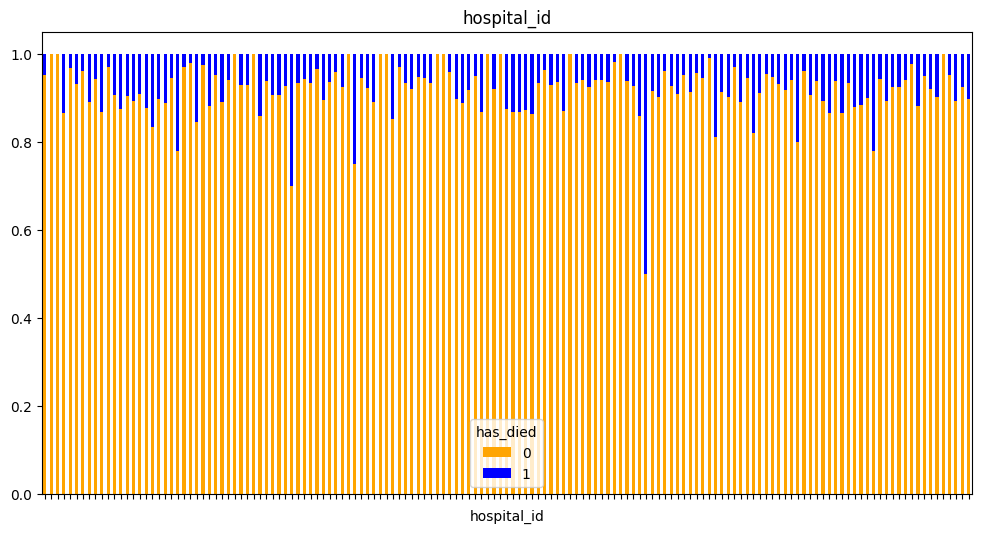
\includegraphics[width=0.9\textwidth]{"./image/dataset/hospital_id_dis.png"}
  \caption{Percentage of Death in Different Hospital}
  \label{fig:hospital}
\end{figure}

\begin{figure}[ht]
  \centering
  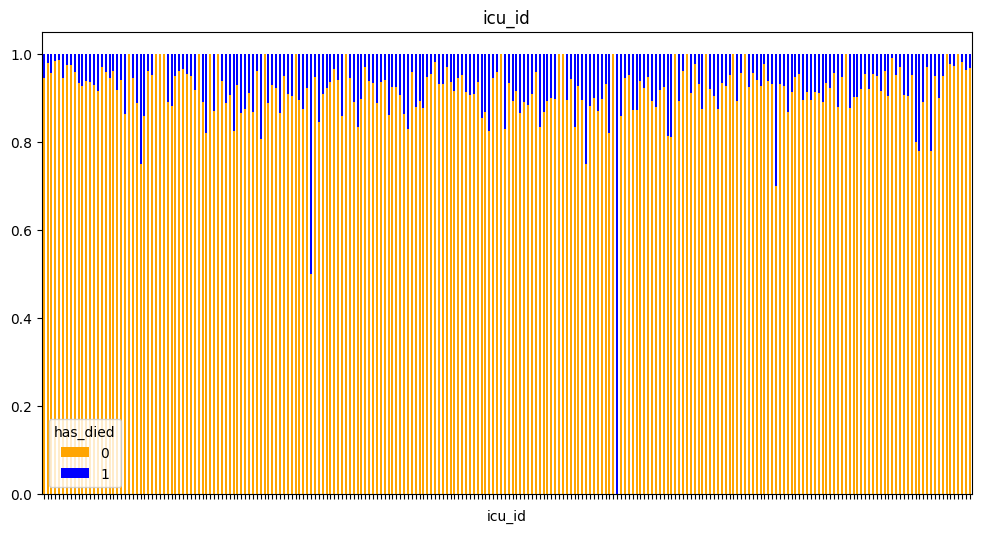
\includegraphics[width=0.9\textwidth]{"./image/dataset/icu_id_dis.png"}
  \caption{Percentage of Death in Different ICU}
  \label{fig:icu}
\end{figure}

From the figure \ref{fig:hospital} and figure \ref{fig:icu}, 
we can see that some of the hostipal and icu have higher death rate than others.
So it's reasonable to assume that the hostipal and icu information are related to the result of death in this dataset,
and it is necessary to keep these features. \\

Since there are some missing values in the categorical features, 
so we can first analyze the relationship between missing values and result of death,
and then decide the way to transform the missing values.
First, I analyze the percentage of missing values in each feature in figure \ref{fig:missing_cat}.
From the figure, we can see that the missing values accounts for proportion of 0.75\% to 1.75\%
in most of the categorical features, now we can look into the 
features with high percentage of missing values.

\begin{figure}[ht]
  \centering
  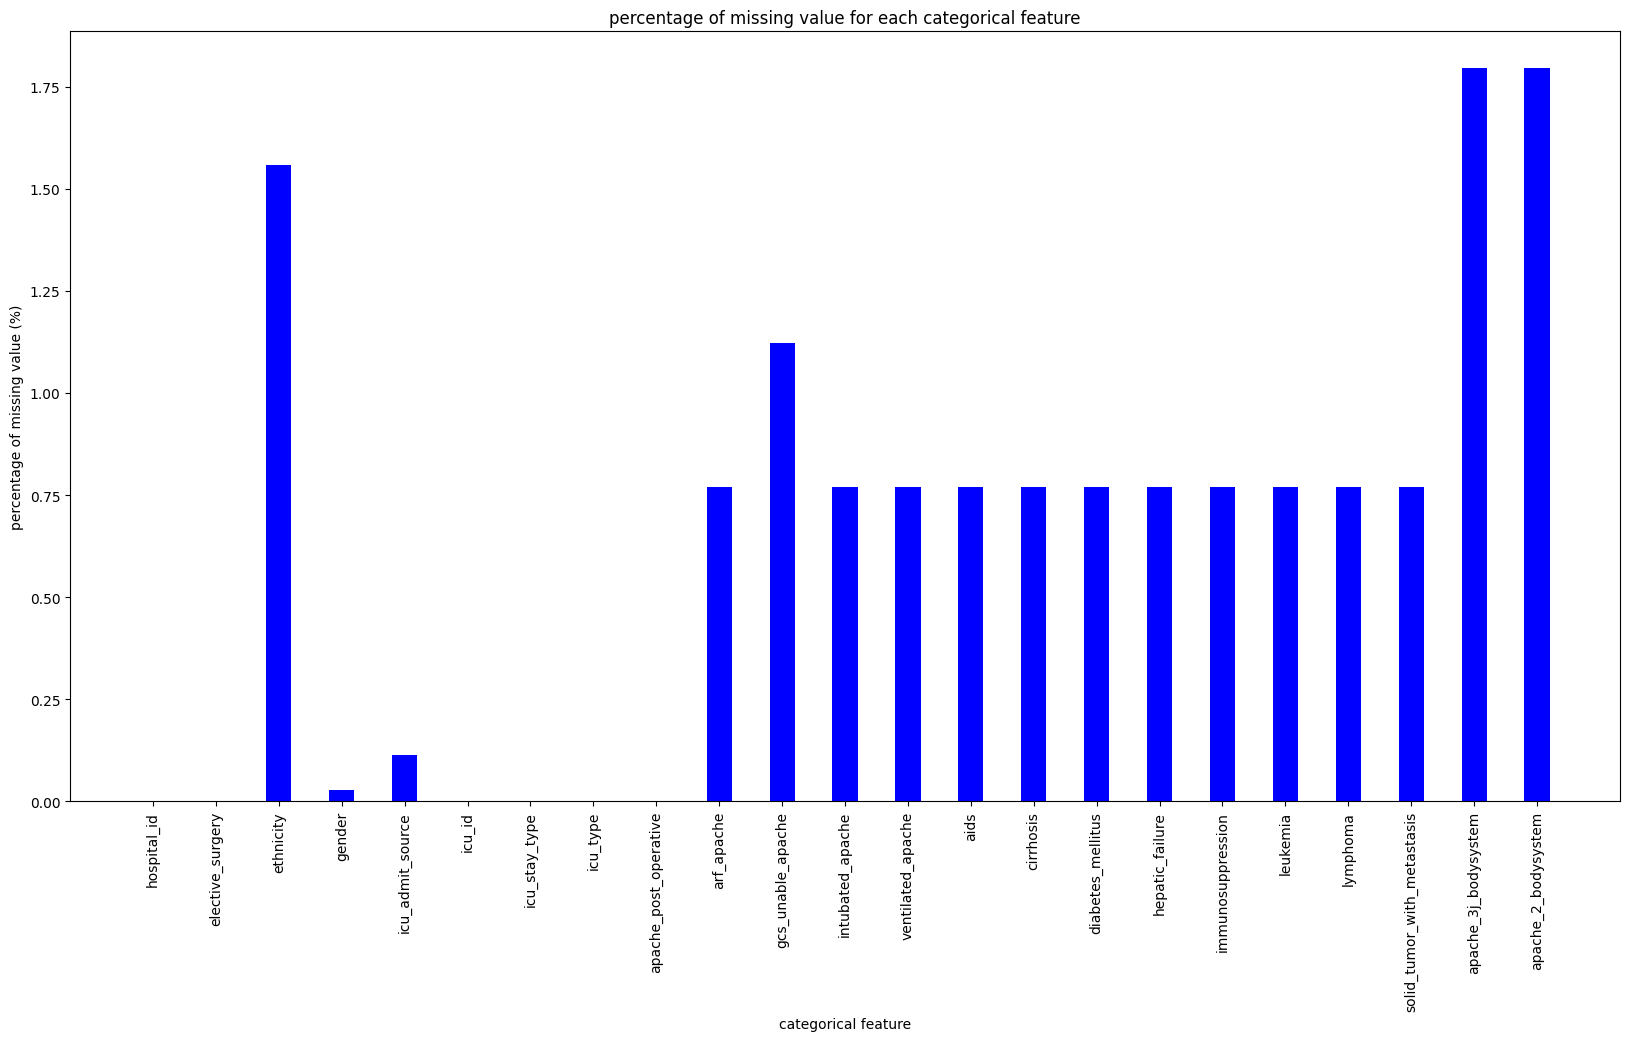
\includegraphics[width=0.9\textwidth]{"./image/dataset/cat_nan_percentage.png"}
  \caption{Percentage of Missing Values in Categorical Features}
  \label{fig:missing_cat}
\end{figure}

For feature \emph{apache\_2\_bodysystem} and \emph{apache\_3j\_bodysystem} and \emph{ethnicity},
the relationship between missing values and death rate is shown in 
figure \ref{fig:apache_2}, figure \ref{fig:apache_3j} and figure \ref{fig:ethnicity}
From the figure, we can see that the missing values 
in these three features still contains some information about the result of death,
so it's not reasonable to simply drop these missing values.
For the rest of categorical features that also contains missing values,
the missing values are also accounts for a small proportion of death rate.
Although these related death result represents a very small proportion of the whole dataset,
it's still necessary to keep these missing values to avoid losing important information.


\begin{figure}[ht]
  \centering
  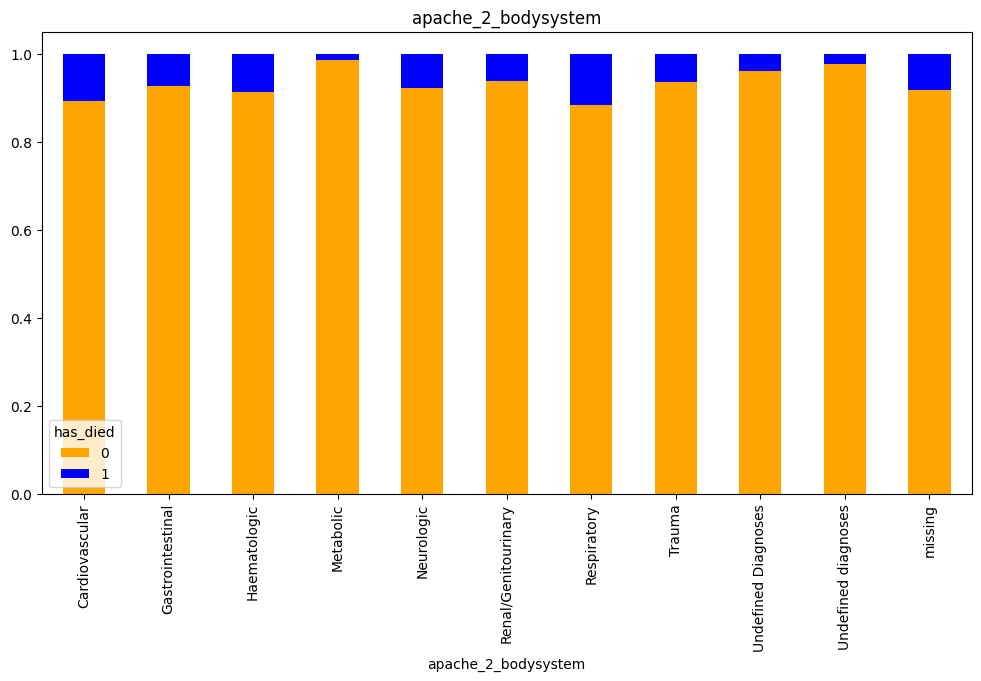
\includegraphics[width=0.62\textwidth]{"./image/dataset/apache_2_dis.png"}
  \caption{Percentage of Death in Different apache\_2\_bodysystem}
  \label{fig:apache_2}
\end{figure}

\begin{figure}[ht]
  \centering
  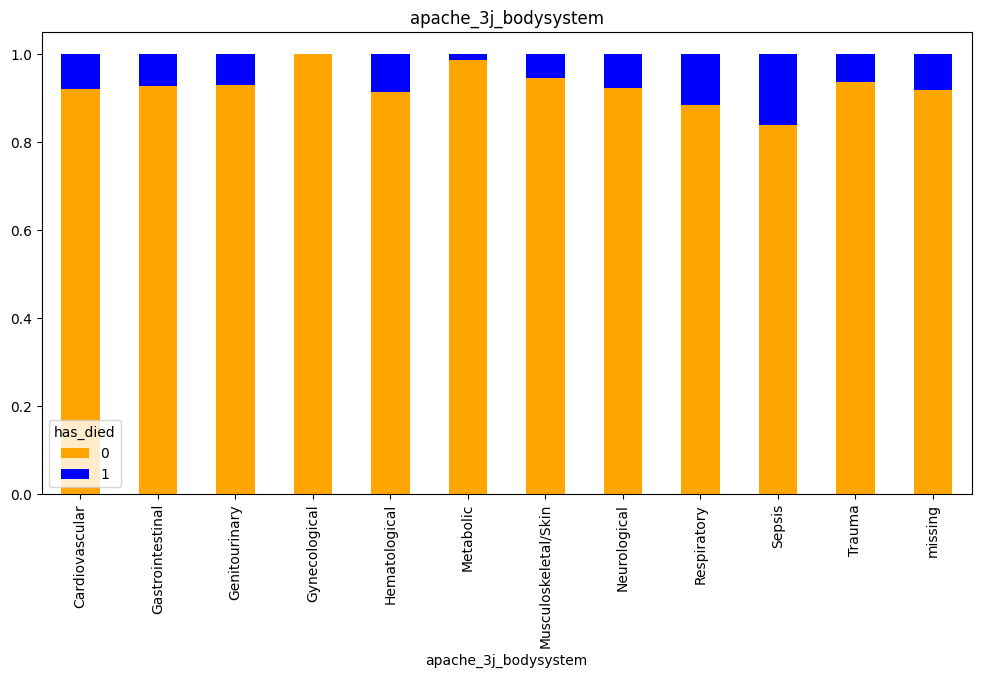
\includegraphics[width=0.62\textwidth]{"./image/dataset/apache_3j_dis.png"}
  \caption{Percentage of Death in Different apache\_3j\_bodysystem}
  \label{fig:apache_3j}
\end{figure}

\begin{figure*}[ht]
  \centering
  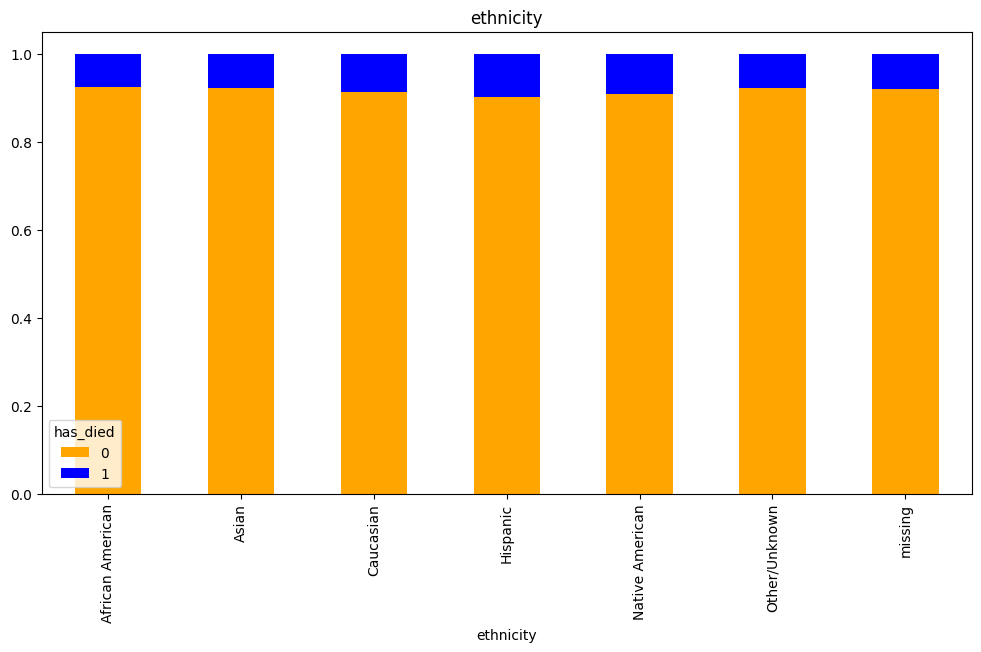
\includegraphics[width=0.62\textwidth]{"./image/dataset/ethnicity_dis.png"}
  \caption{Percentage of Death in Different ethnicity}
  \label{fig:ethnicity}
\end{figure*}

\clearpage

\subsubsection{Numerical Features}

For numerical features, I first analyze the percentage of 
missing values in figure \ref{fig:num_nan_percentage}.
From the figure we can see the proportion of missing values in most of numerical features
is much higher than the categorical features.
For further analysis, I fill the missing values with the mean value of each feature,
which can minimize the impact of missing values.

\begin{figure}[h]
  \centering
  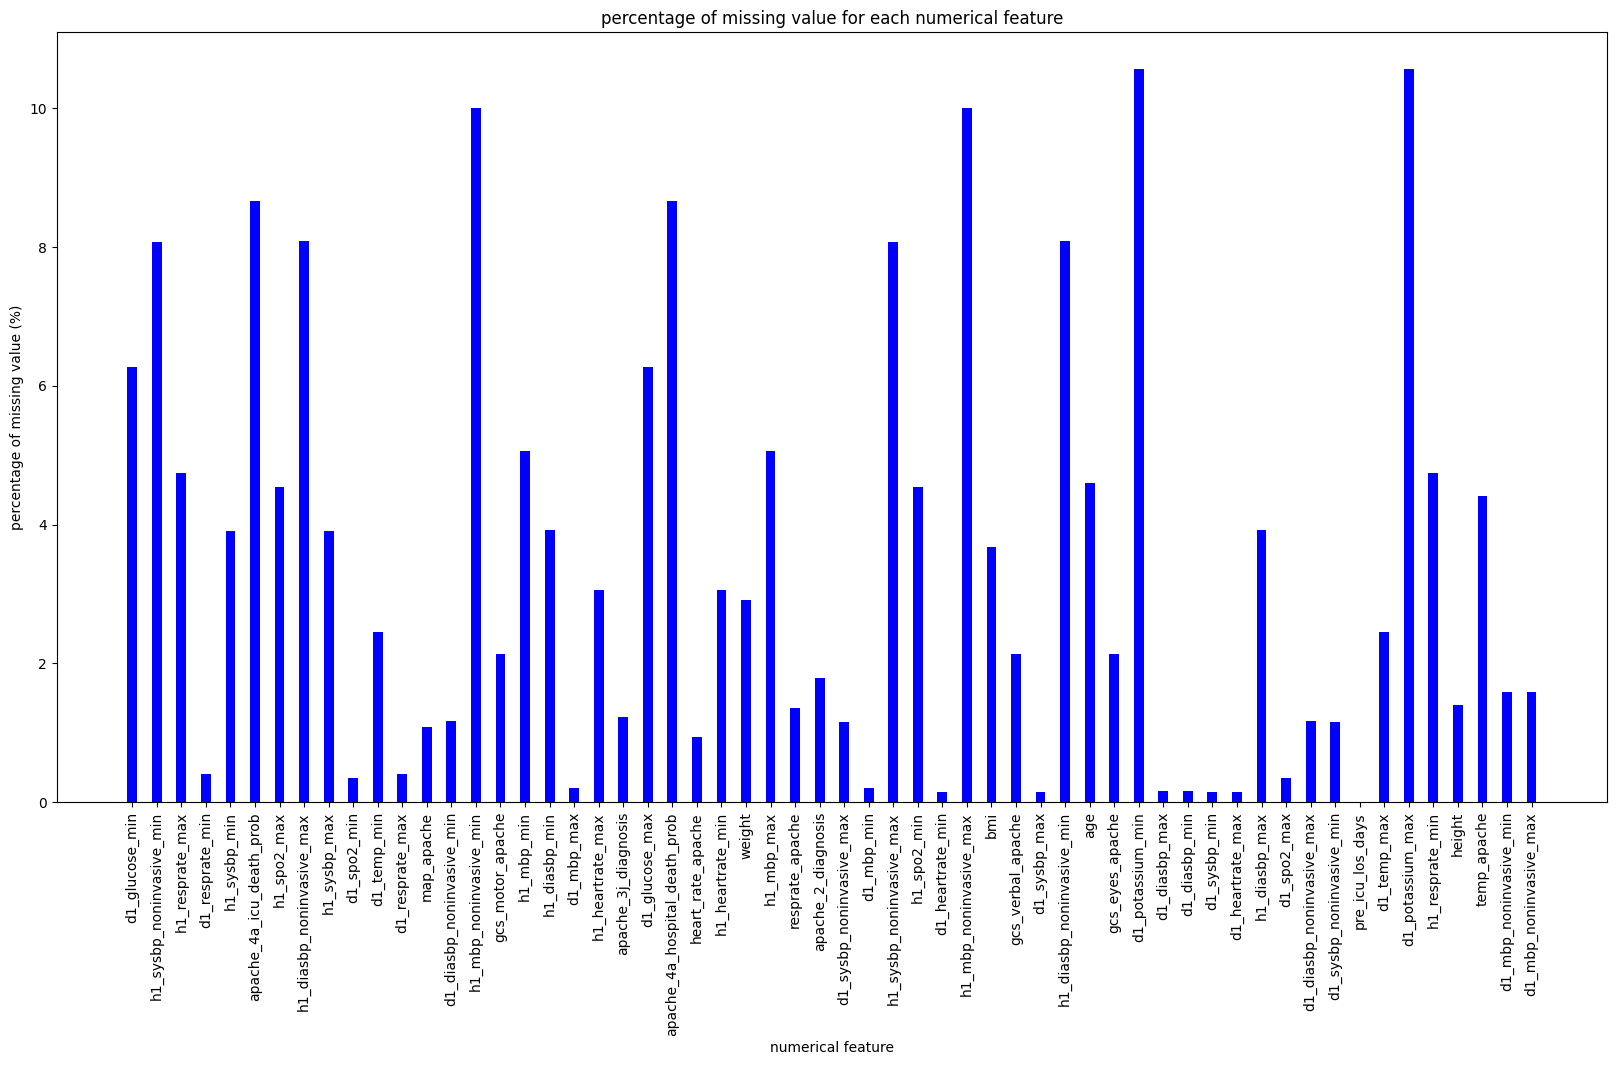
\includegraphics[width=0.9\textwidth]{"./image/dataset/num_nan_percentage.png"}
  \caption{Percentage of Missing Values in Numerical Features}
  \label{fig:num_nan_percentage}
\end{figure}

Figure \ref{fig:bmi} show the distribution of bmi in different result of death.
From the figure, we can see the trend of bmi value among our dataset,
and the percentage of death is quite similar in different bmi value.
An other interesting discovery is that there are some abnormal distribution near the bmi value 70,
which I think is the outlier of this dataset at the first glance.
However, after further analysis, I found that the same distribution trend can be found in
feature \emph{weight} from figure \ref{fig:weight},
which means the abnormal distribution may be casued by realistic reasons,
such as some diagnosis or treatment may cause the patient to gain weight.

\begin{figure}[h]
  \centering
  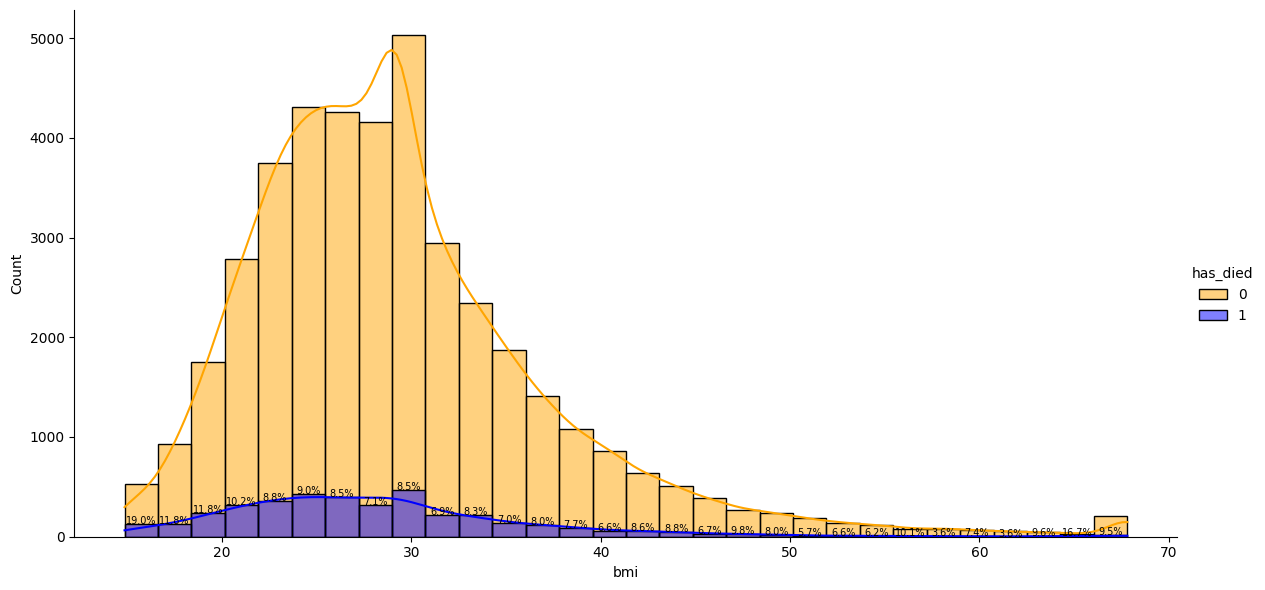
\includegraphics[width=0.7\textwidth]{"./image/dataset/bmi_dis.png"}
  \caption{Distribution of bmi}
  \label{fig:bmi}
\end{figure}

\begin{figure}[h]
  \centering
  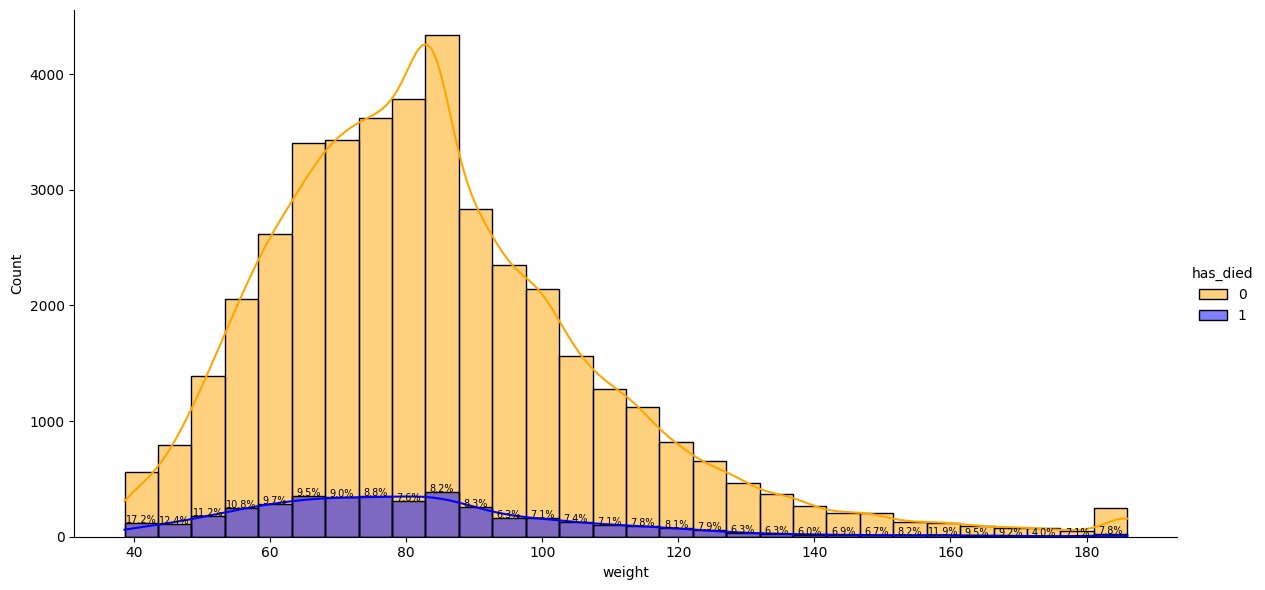
\includegraphics[width=0.7\textwidth]{"./image/dataset/weight_dis.png"}
  \caption{Distribution of weight}
  \label{fig:weight}
\end{figure}

\newpage

The discovery about outliers can be found in 
feature \emph{apache\_4a\_hospital\_death\_prob} and \emph{apache\_4a\_icu\_death\_prob}.
From figure \ref{fig:apache_4a_hospital_death_prob} and figure \ref{fig:apache_4a_icu_death_prob},
we can see there are some negative values in these two features,
which is obviously the outliers when representing the probability of death.
To dealing with these outliers, I replace them with NaN values and use imputation for restoring,
expect this operation can let the new value be more realistic.
The details of imputation will be mentioned in the following section.

\begin{figure}[h]
  \centering
  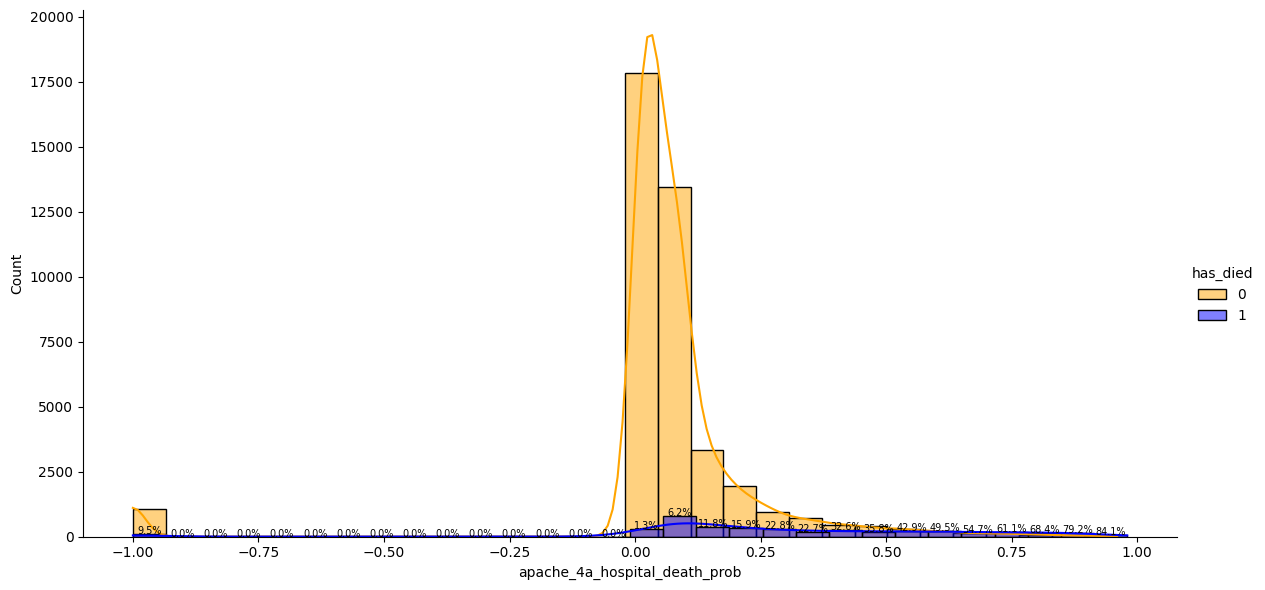
\includegraphics[width=0.7\textwidth]{"./image/dataset/hospital_death_prob_dis.png"}
  \caption{Distribution of apache\_4a\_hospital\_death\_prob}
  \label{fig:apache_4a_hospital_death_prob}
\end{figure}

\begin{figure}[h]
  \centering
  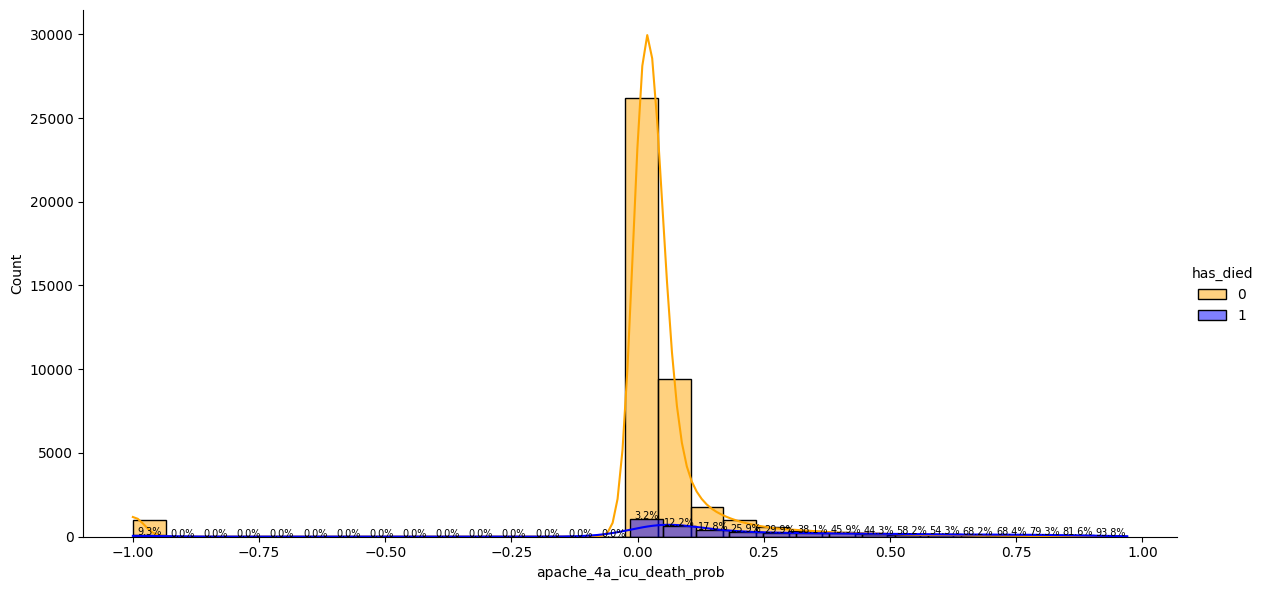
\includegraphics[width=0.7\textwidth]{"./image/dataset/icu_death_prob_dis.png"}
  \caption{Distribution of apache\_4a\_icu\_death\_prob}
  \label{fig:apache_4a_icu_death_prob}
\end{figure}

\subsubsection{Imbalanced Data}

For this dataset, the proportion of death is only 8.63\%, 
which means the dataset is highly imbalanced (see Figure \ref{fig:label_dis}).
Since the imbalanced data will lead to frequency bias on the learning model,
so there are some solutions for training on a imbalanced data,
which will be concluded in the following section.

\begin{figure}[h]
  \centering
  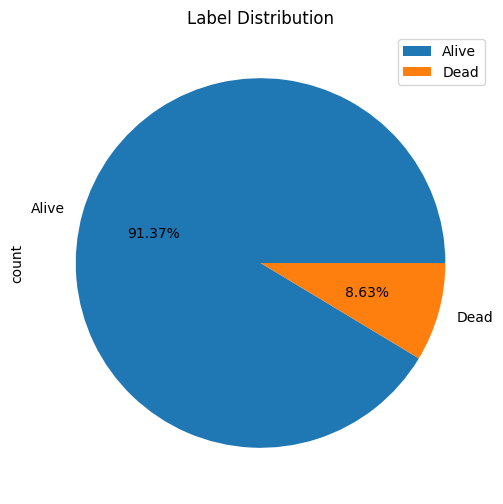
\includegraphics[width=0.6\textwidth]{"./image/dataset/alive_dead_dis.png"}
  \caption{Distribution of Label}
  \label{fig:label_dis}
\end{figure}

\section{Data Preprocessing}

\subsection{Feature Encoding}

For this dataset, I tried several encoding method for categorical feature transformation.

\subsubsection{One-hot Encoding}

One-hot encoding is the most common way to transform categorical features,
but for the features with multiple categories, it will lead to sparse embedded data with high dimension,
which ccause the curse of dimensionality.

\subsubsection{Frequency Encoding}

Frequency Encoding is an better way to avoid the curse of dimensionality comparing to one-hot encoding.
The idea of frequency encoding is to replace the category value with the frequency of that category in the dataset.
But for the features that each category with similar frequency, it will cause the problem of information loss.

\subsubsection{Target Encoding}

For target encoding, it will replace the category value with the mean value of the target value in that category.
the advantage of target encoding is that it shows the relationship between each category and target value.
But it may cause the problem of overfitting since the label information is directly used in the training process.

\subsection{Imputation}

For imputation, I tried several imputation methods to restore the missing values in the dataset.
Since the missing values of categorical features accounts for a large proportion of the whole dataset,
so it's important to find a proper way to restore the missing values.

\subsubsection{Most-Frequent Imputation}

Most-frequent imputation is a common way to restore the missing values of categorical features.
Since for each categorical features, it's highly possible that the actual value is the most frequent value.

\subsubsection{Mean / Median Imputation}

For numerical features, mean / median imputation is a reasonable way to restore the missing values.
Since the mean / median value can be close to the actual value of the missing values.

\subsubsection{KNN Imputation}

For the imputation techniques mentioned above, they are all completed according to the same single feature of the dataset.
But it's more reasonable to restore the missing values according to the relationship between different instances,
which considers other features when measuring the similarity between instances.
KNN imputation is such a method like that, which first find the k nearest instances of the one with mmissing values,
and then use mean value to restore the missing values.
The advantage of KNN imputation is quite obvious since the basis of imputation is more accurate,
but it also has the disadvantage of time complexity comparing to the other two methods.

\subsection{Disscussion of Encoding and Imputation Method}

For the imputation and encoding method mensioned above, I tried several combinations of them,
and the result is shown in the table \ref{tab:encoding_imputation}, 
which shows the internal K-Fold average Macro F1 score and AUROC score of each combination.
The \emph{Simple} imputation method means applying the median imputation for numerical features,
and most-frequent imputation for categorical features.
Experiments are all following the same training and testing process mensioned in experiment section,
and the best result of each combination is shown in the table.
We can see that KNN imputation method can reach higher performance than Simple imputation method,
which means using the relationship between instances can help the model to learn better.
For the encoding method, target encoding can reach higher performance than frequency encoding,
which means the relationship between category and label is important for this dataset.
According to the result, I choose the combination of \emph{Target} encoding and \emph{KNN} imputation for the following experiment.

\begin{table}[h]
  \centering
  \begin{tabular}{|c|c|c|c|}
    \hline
    Encoding & Imputation & Macro F1 & AUROC \\
    \hline
    Frequency & Simple & 0.728 & 0.734 \\
    \hline
    Frequency & KNN & 0.728 & 0.737 \\
    \hline
    Target & Simple & 0.730 & 0.737 \\
    \hline
    Target & KNN & 0.732 & 0.740 \\
    \hline
  \end{tabular}
  \caption{Evaluation of Encoding and Imputation Method}
  \label{tab:encoding_imputation}
\end{table}

Note: The result of this table are all evaluated on Persenal Computer (spec below),
so the result may be slightly different from the result of the following section,
which is evaluated on Kaggle Platform.

\begin{itemize}
  \item OS: Windows 10 22H2
  \item CPU: Intel(R) Xeon(R) CPU E3-1231 v3 @ 3.40GHz
  \item python: 3.12.0
\end{itemize}

\section{Feature Selection}

Feature selection is an important step in data preprocessing,
which can reduce the dimension of training data and help the model reach higher performance.

\subsection{Correlation Coefficient}

Furthermore, we can also use correlation coefficient to find the relationship between each
feature and result of death, and then select the features that is highly related to the label.
When selecting the features, we can also consider the correlation between features to avoid
the problem of multicollinearity.
For the correlation of each feature and label, I use biserial correlation coefficient to measure the relationship,
which is suitable for the relationship between continuous and binary variables, figure \ref{fig:biserial_correlation} shows the result.

\begin{figure}[h]
  \centering
  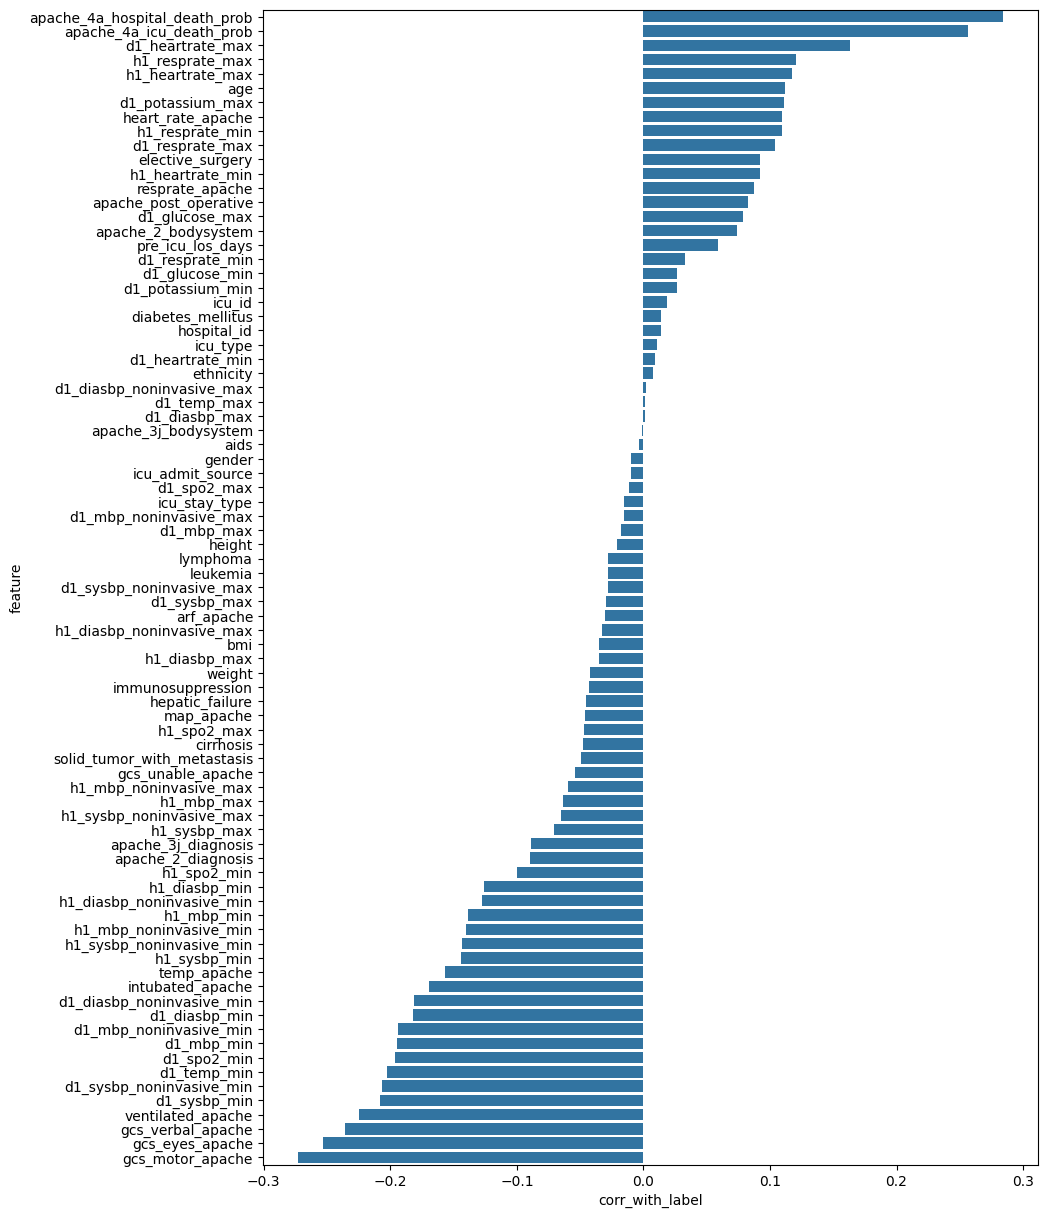
\includegraphics[width=0.9\textwidth]{"./image/biserial_corr.png"}
  \caption{Biserial Correlation Coefficient}
  \label{fig:biserial_correlation}
\end{figure}

Pearson correlation coefficient is used to measure the correlation between continuous variables,
so I use it for finding the correlation between features, figure \ref{fig:pearson_correlation} shows the result.

\begin{figure}[h]
  \centering
  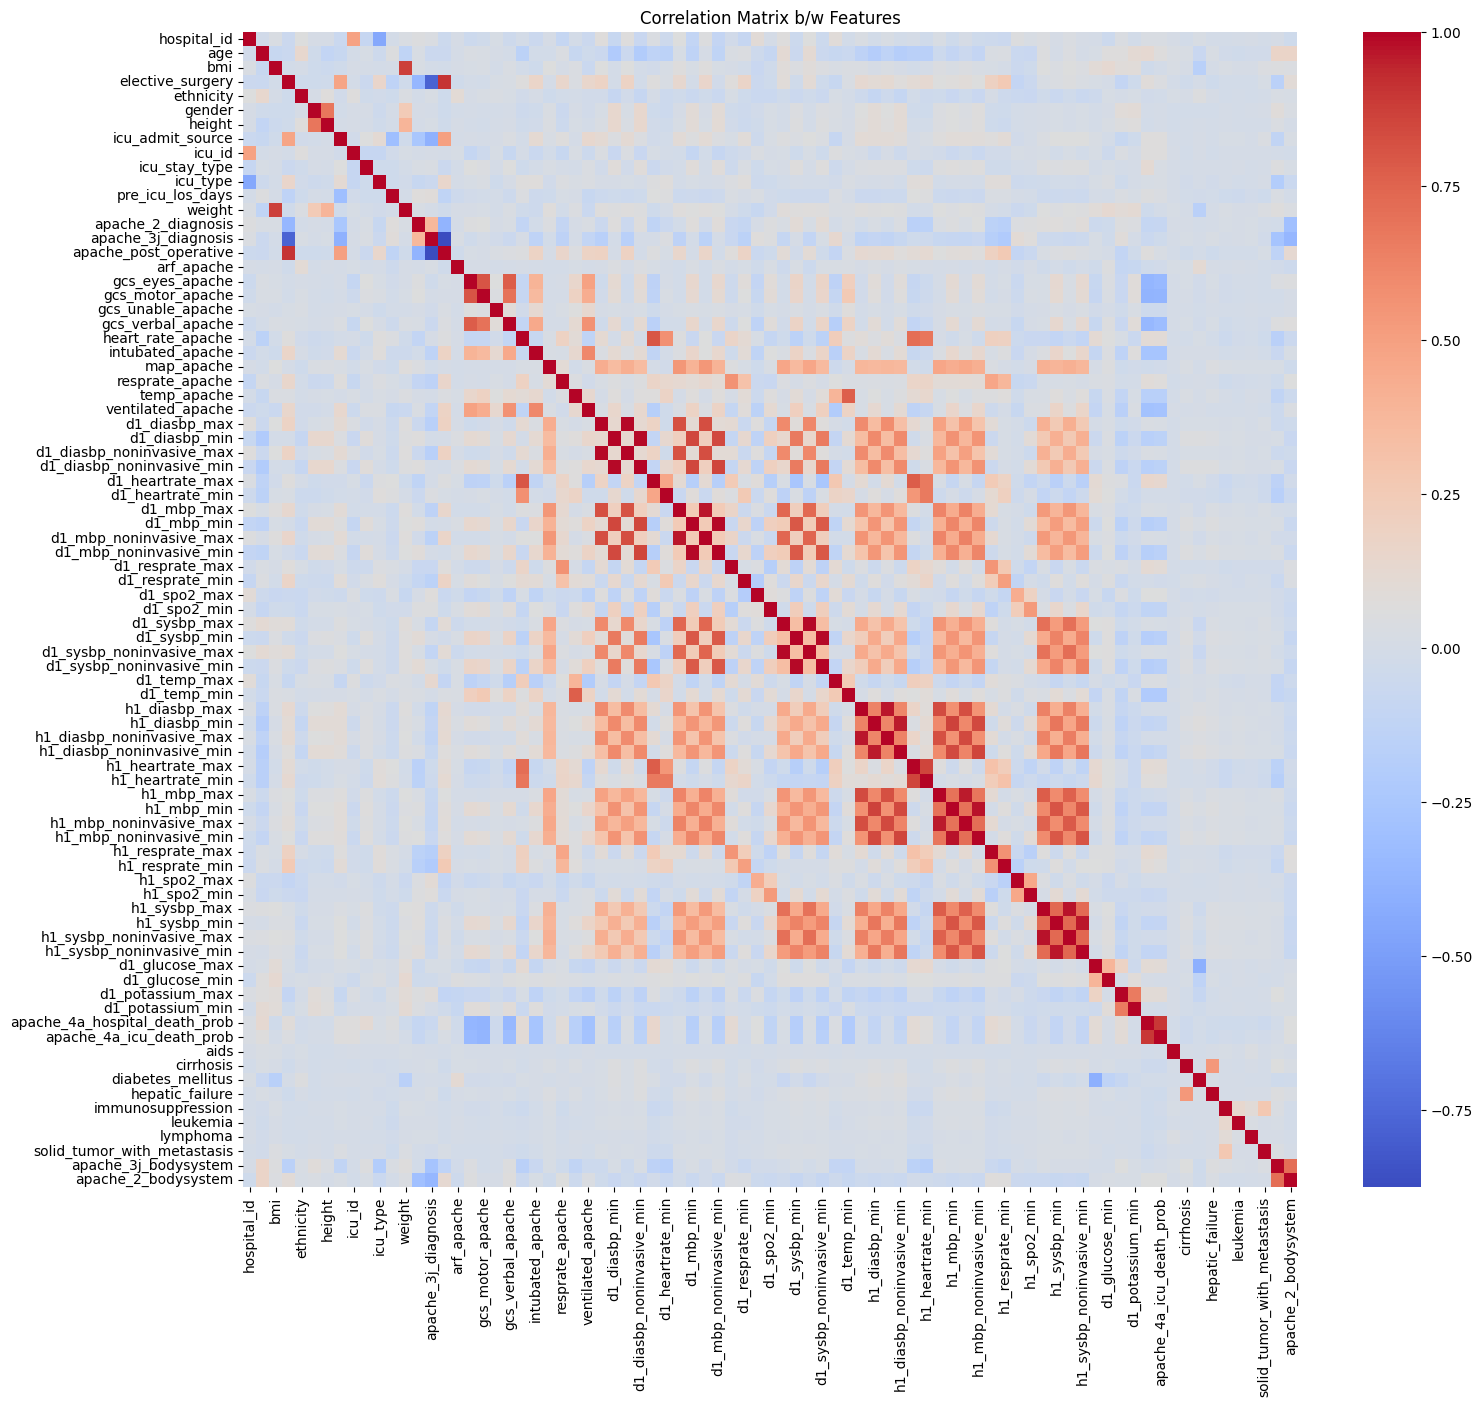
\includegraphics[width=1.0\textwidth]{"./image/feature_corr.png"}
  \caption{Pearson Correlation Coefficient}
  \label{fig:pearson_correlation}
\end{figure}

\clearpage

\subsection{Sharpley Value}

Sharpley value is a metric for measuring the importance of each feature,
which is suitable for the classification problem.
The idea of Sharpley value is to calculate the difference of the model performance
before and after removing the feature.
The feature with higher Sharpley value means it has higher impact on the model performance.
Figure \ref{fig:shap_mean_before} and figure \ref{fig:shap_value_before} 
shows the Sharpley value of top20 features before selection.

\begin{figure}[ht]
  \centering
  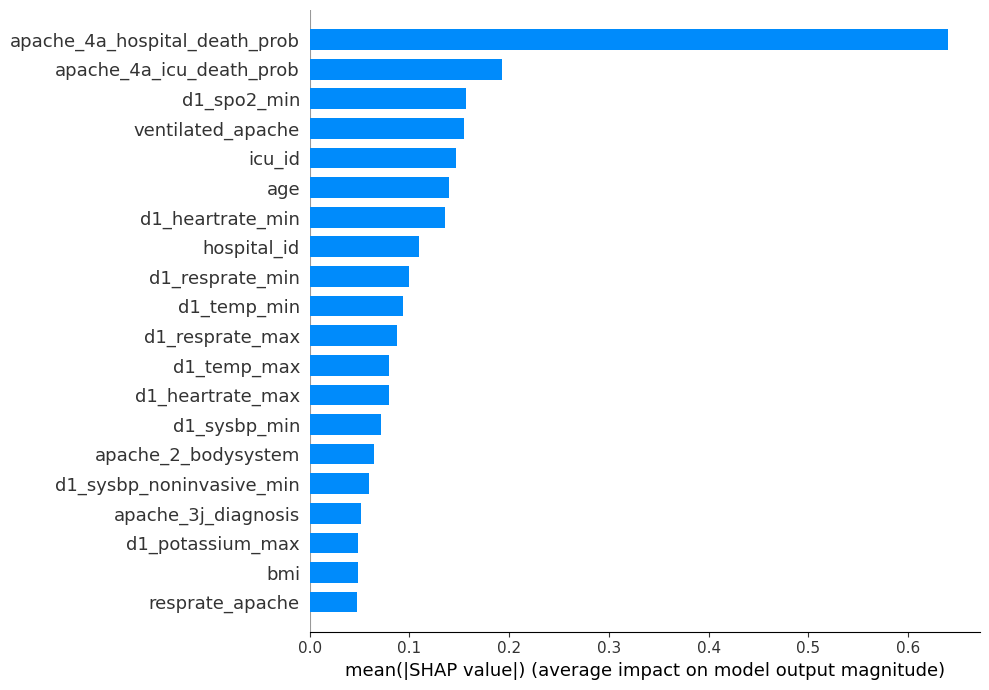
\includegraphics[width=0.7\textwidth]{"./image/shap_mean_before.png"}
  \caption{Top20 Mean Sharpley Value Before Selection}
  \label{fig:shap_mean_before}
\end{figure}

\begin{figure}[ht]
  \centering
  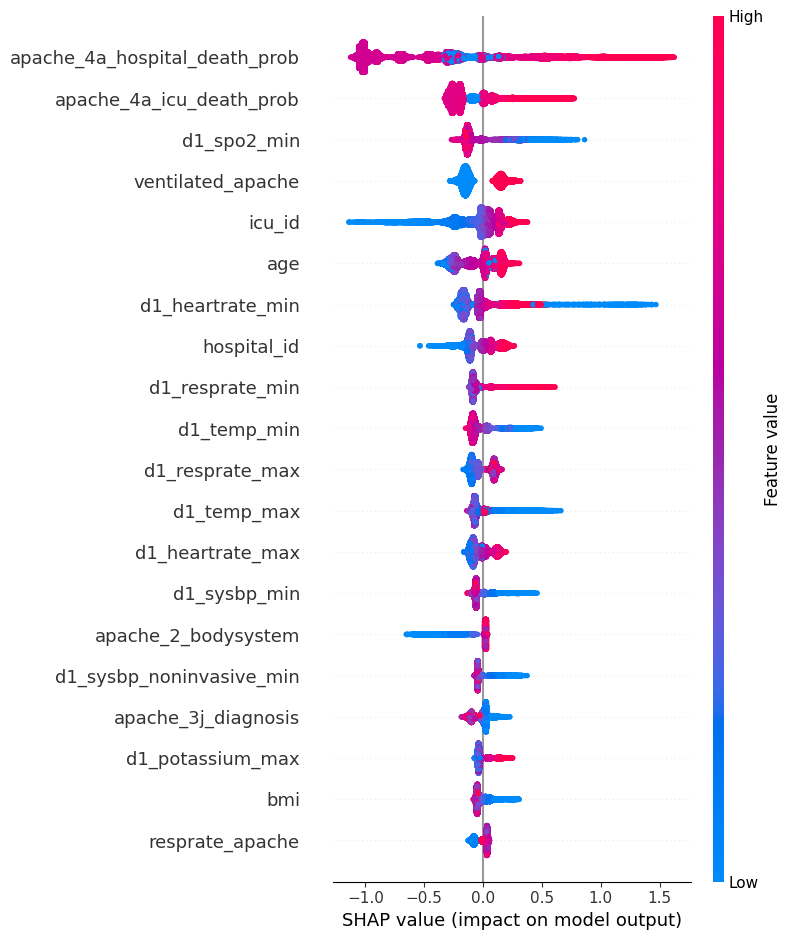
\includegraphics[width=0.5\textwidth]{"./image/shap_value_before.png"}
  \caption{Top20 Sharpley Value Before Selection}
  \label{fig:shap_value_before}
\end{figure}

\clearpage

In the figure, we can see the features with higher Sharpley value,
such as \emph{apache\_4a\_hospital\_death\_prob}, \emph{apache\_4a\_icu\_death\_prob},
\emph{d1\_spo2\_min}, etc. 
These features are also have high correlation with the result of death,
but we cannot simply choose these features since they might cause
multicollinearity problem with other features that also have high Sharpley value.
So I consider Sharpley value, biserial correlation to find the features that 
are highly related to the result of death and contribute greatly to the model performance,
And remove the features that are highly correlated with other features using Pearson correlation coefficient.
Additionally, the dataset is highly imbalanced, so I use undersampling to balance the dataset for selecting features.
Since the sampling method are totally random, so I repeat the sampling process for several times,
and choose the features that are selected for most of the time.
Finally I choose 22 important features for training the model.
Figure \ref{fig:shap_mean_after} and figure \ref{fig:shap_value_after} shows the Sharpley value of each feature after feature selection.

\begin{figure}[h]
  \centering
  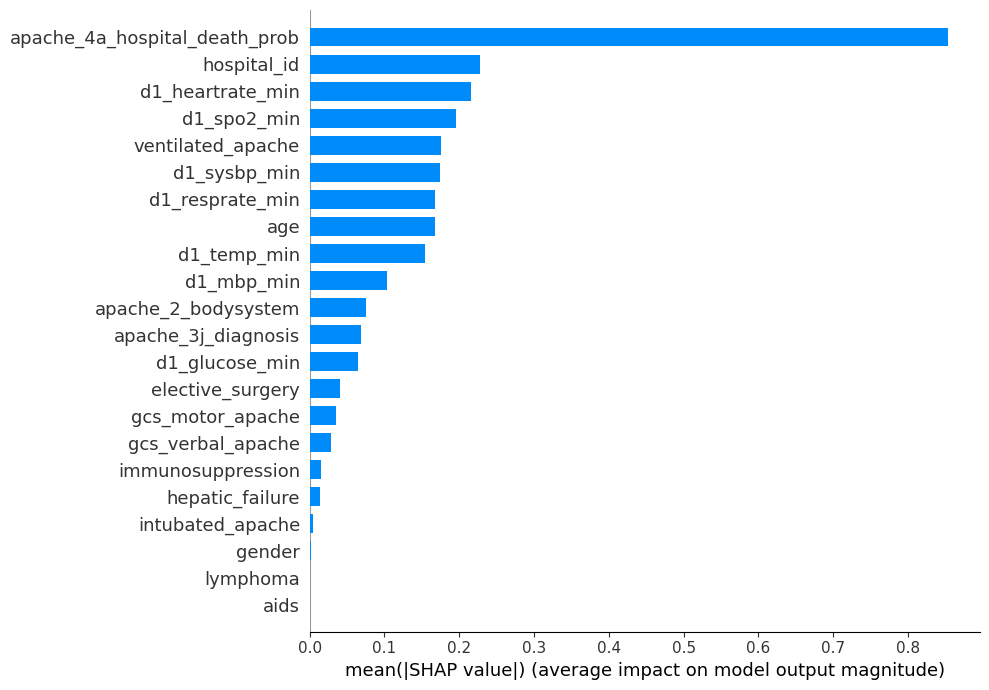
\includegraphics[width=0.9\textwidth]{"./image/shap_mean.png"}
  \caption{Mean Sharpley Value After Selection}
  \label{fig:shap_mean_after}
\end{figure}

\begin{figure}[h]
  \centering
  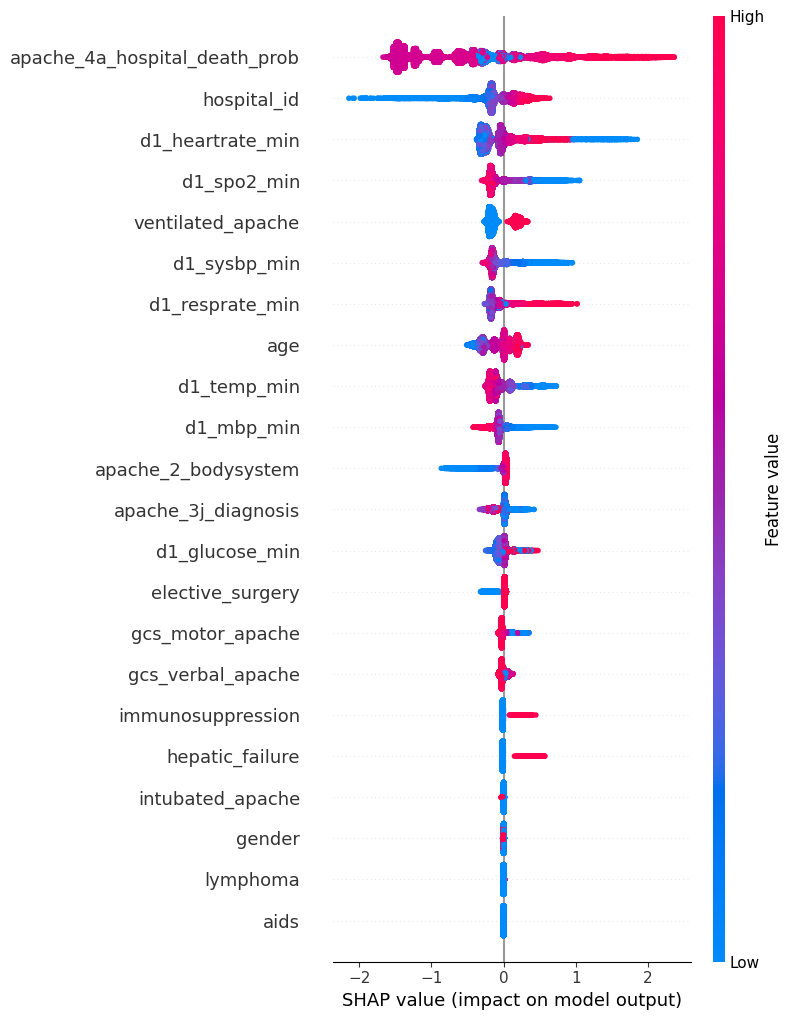
\includegraphics[width=0.8\textwidth]{"./image/shap_value.png"}
  \caption{Sharpley Value After Selection}
  \label{fig:shap_value_after}
\end{figure}

Now we can see the features with higher Sharpley value and biserial correlation coefficient are selected.
Some features with high correlation with other features are removed,
such as \emph{apache\_4a\_icu\_death\_prob}, although it has high Sharpley value,
but it has high correlation with \emph{apache\_4a\_hospital\_death\_prob} 
(according to figure \ref{fig:pearson_correlation}), so it's removed.
Other features are included in the feature selection for obvious reasons,
such as \emph{hospital\_id}, which we can see from figure \ref{fig:hospital} that
the death rate differ dramatically in different hospital.
There are some features that are selected but they don't 
have high correlation with the result of death or Sharpley value,
such as \emph{gender}, \emph{lymphoma} and \emph{aids}.
So I think I can try further feature selection to find the best combination of features.
In order to do that, I use the \emph{SequentialFeatureSelector} function from \emph{mlxtend} package,
which can find the best combination of features according to the given evaluation metrics (Marco F1 score).

\clearpage

\section{Classification Model}

\subsection{Model Selection}

The classification model I used for this assignment is XGBoost\cite{chen2016xgboost},
which combines the advantages of both bagging and boosting.
For bagging, it uses the idea of random forest to train 
multiple weak learners (trees) with different subset of training data,
and each new tree will correct the error of the previous tree, 
which is the idea of boosting.
The advantage of XGBoost is that it can avoid the overfitting problem of boosting
with the regularization term and pruning technique, which can also reduce the time complexity.

\subsection{Hyperparameter Tuning}

For hyperparameter tuning, I use the \emph{GridSearchCV} function from \emph{sklearn} package.
With this function, I can find the hyperparameter profile that can reach the highest performance
within the internal K-fold cross validation.

\subsection{Training with Imbalanced Data}

For imbalanced data, I tried oversampling method such as SMOTE,
but it did not improve the performance of the model,
worsely, it will cost more time for training since the dataset is almost 2 times larger.
So I choose to adjust class weight to deal with this problem.
The idea of adjusting class weight is to increase the weight of the minority class,
which can let the model pay more attention to the minority class.
I tried several weight ratio, and find that the ratio 3:1 can reach the best performance.

\subsection{Model Evaluation}

For model evaluation, I follow the instruction of the assignment, which uses the Macro F1 score and AUROC score
as the evaluation metrics. These two metrics are both suitable for imbalanced data,
which can truely reflect the performance of the model.

\section{Experiment}

\subsection{Experiment Environment}

\begin{itemize}
  \item Platform: Kaggle Notebook
  \item Python 3.10.2
  \begin{itemize}
    \item pandas 2.0.3
    \item sklearn 1.2.2
    \item mlxtend 0.23.0
    \item xgboost 2.0.2
  \end{itemize}
\end{itemize}

\subsection{Experiment Setting}

\begin{itemize}
  \item k = 5 for KNN imputation
  \item k = 5 for internal K-Fold cross validation (split by \emph{sklearn.model\_selection.KFold})
  \item XGBoost (hyperparameter found by GridSearchCV)
  \begin{itemize}
    \item colsample: 0.8
    \item gamma: 0.1
    \item learning rate: 0.1
    \item max\_depth: 3
    \item min\_child\_weight: 1
    \item n\_estimators: 12000
    \item random\_state: 42
    \item scale\_pos\_weight: 3
  \end{itemize}
  \item \emph{SequentialFeatureSelector} from \emph{mlxtend} package (hyperparameter found by GridSearchCV)
  \begin{itemize}
    \item k\_features: 15
  \end{itemize}
\end{itemize}

\subsection{Experiment Result}

\begin{itemize}
  \item Internal K-Fold (Running on Kaggle Notebook)
  \begin{itemize}
    \item Macro F1 score: 0.723
    \item AUROC score: 0.730
  \end{itemize}
  \item Test data (Evaluated by Kaggle Competition)
  \begin{itemize}
    \item Marco F1 score: 0.735
  \end{itemize}
\end{itemize}

Note: The score of this section is all evaluated on Kaggle Platform,
so the result may be slightly different from the result of table \ref{tab:encoding_imputation}.

\subsection{How to Reproduce the Result}

\begin{itemize}
  \item Import the ipynb file to Kaggle Notebook
  \item Modified the path of dataset in the fourth cell (file name) last cell (path)
  \item Run the code in order
  \item The result will be shown in the last cell
\end{itemize}

\endgroup

\bibliographystyle{unsrt} % We choose the "plain" reference style
\bibliography{reference} % Entries are in the "references.bib" file

\end{document}